\subsubsection{Pixel Buffer}
\label{sec:pixel_buffer}

The pixel buffer for the video-out port holds the data (color) for each pixel that
will be displayed.  As illustrated in Figure \ref{fig:video_coord}, the
pixel buffer provides an image resolution of 
160 $\times$ 120 pixels, with the coordinate 0,0 being at the top-left corner of the image. 
Since the video-out port supports the screen resolution of 640 $\times$ 480, each of the
pixel values in
the pixel buffer is replicated 4 times in both the {\it x} and {\it y} dimensions when it is being
displayed on the screen.

\begin{figure}[h!]
   \begin{center}
       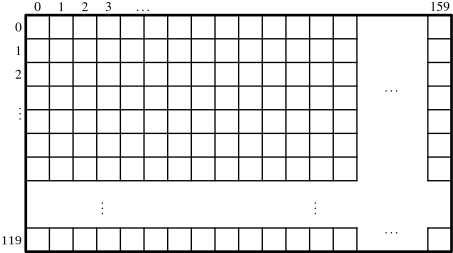
\includegraphics{../../../common/figs/Media_FPGA_Video_Coord_160120.pdf}
   \end{center}
   \caption{Pixel buffer coordinates.}
	\label{fig:video_coord}
\end{figure}

Figure \ref{fig:pixels}$a$ shows that each pixel color is represented as a 16-bit halfword, 
with five bits for the blue and red 
components, and six bits for green.  As depicted in part $b$ of Figure \ref{fig:pixels}, 
pixels are addressed in the pixel buffer by 
using the combination of a {\it base} address and an {\it x,y} offset.  In the \systemName~the default
address of the pixel buffer is {\sf 0x\baseAddressOffset 8000000}, which corresponds
to the starting address of the FPGA on-chip memory.  Using this scheme, the pixel at 
location 0,0 has the address {\sf 0x\baseAddressOffset 8000000}, 
the pixel 1,0 has the address {\it base} $+$ (00000000~00000001~0)$_2$ = {\sf 0x\baseAddressOffset 8000002}, 
the pixel 0,1 has the address {\it base} $+$ (00000001~00000000~0)$_2$ = {\sf 0x\baseAddressOffset 8000200},
and the pixel at location 159,119 has the address {\it base} $+$ (1110111 10011111 0)$_2$ = 
{\sf 0x\baseAddressOffset 800EF3E}. 

\begin{figure}[h!]
   \begin{center}
       \includegraphics{../../../common/figs/Media_FPGA_Video_Pixel_Values_16.pdf}
			 \caption*{Pixel values}
			 \vspace{1cm}
			 \includegraphics{../../../common/figs/Media_FPGA_Video_Pixel_Address_16_1.pdf}
			 \caption*{Pixel addresses}
   \end{center}
   \caption{Pixel values and addresses.}
	\label{fig:pixels}
\end{figure}

You can create an image by writing color values into the pixel addresses as described
above. A dedicated {\it pixel buffer controller} continuously reads this pixel 
data from sequential addresses in the corresponding
memory for display on the screen.  You can modify the pixel data at any time, simply
by writing to the pixel addresses. Thus, an image can be changed even when it is in the
process of being displayed.  However, it is also possible to avoid making changes to 
the pixel buffer while it is being displayed, by using the concept of {\it
double-buffering}.  In this scheme, two pixel buffers are involved, called the {\it front} 
and {\it back} buffers, described below.

